\chapter{Simulation and Reconstuction of Events}
\label{ch:sim_reco}

%\section{Proton-Proton Scattering}
%In a proton-proton scattering process, different outcomes are possible. The cross section for one specific outcome is %proportional to the probability that this outcome will happen. The determination of the cross section $\sigma$ can be done in %multiple steps, for example for the top quark pair production with quarks one gets
%\begin{equation}\label{eq:ch_3_ppscatter}
%\sigma_{qq \rightarrow \textrm{t} \bar{\textrm{t}}} = \underbrace{\sum_{j,k}\int \textrm{d}x_j \textrm{d}x_k}_\text{sum initial states} \overbrace{f_j(x_j,\mu^2) f_k(x_k,\mu^2) }^\text{parton distribution functions} \ \underbrace{\hat{\sigma}(q_j q_k \rightarrow \textrm{t} \bar{\textrm{t}})}_\text{hard scattering process}\  \otimes \  \textrm{hadronization} \quad .
%\end{equation}
%First one has to sum over all initial states, a parton distribution function gives the probability to find a certain particle. The hard scattering process describes the transitions from the initial particles to the final state and the hadronization forms color neutral objects. In this section these steps will be described in more detail. 

All the available information about a particle collision is the measured deposited energy of each detector component. Together with some results of the online reconstruction e.g. trigger signals, this information is stored for further reconstruction. In the offline reconstruction, physical objects like electrons and hadrons are reconstructed. To compare the measured data with the theory prediction, or to investigate the efficiencies and robustness of algorithms, a simulation is needed. In this chapter the simulation process is described followed by an explanation of the reconstruction process. Additionally, methods to correct differences between the measured data, shortly denoted as data, and the simulation are summarized. 


\section{Event Simulation}
The simulation is done using as much theory input as possible. In the same order as the physical process, from the proton-proton scattering to the outgoing particles, one propagates the simulation. Due to insufficient theoretical descriptions, phenomenological models are used when necessary. After the outgoing particles are generated, the interaction with the detector materials is simulated. The emulation for the readout electronics generates signals that have the same signature as the data. 

\subsection{Proton-Proton Scattering}
A proton-proton scattering process leads to the production of a specific final state. The cross section is proportional to the probability to produce this final state. The determination of the cross section $\sigma$ is done in multiple steps, these steps are outlined in figure \ref{fig:ch_3_scattering} and explained in the following.

%FIXME plot zu proton-proton scattering like Husemanns
\begin{figure}
\centering
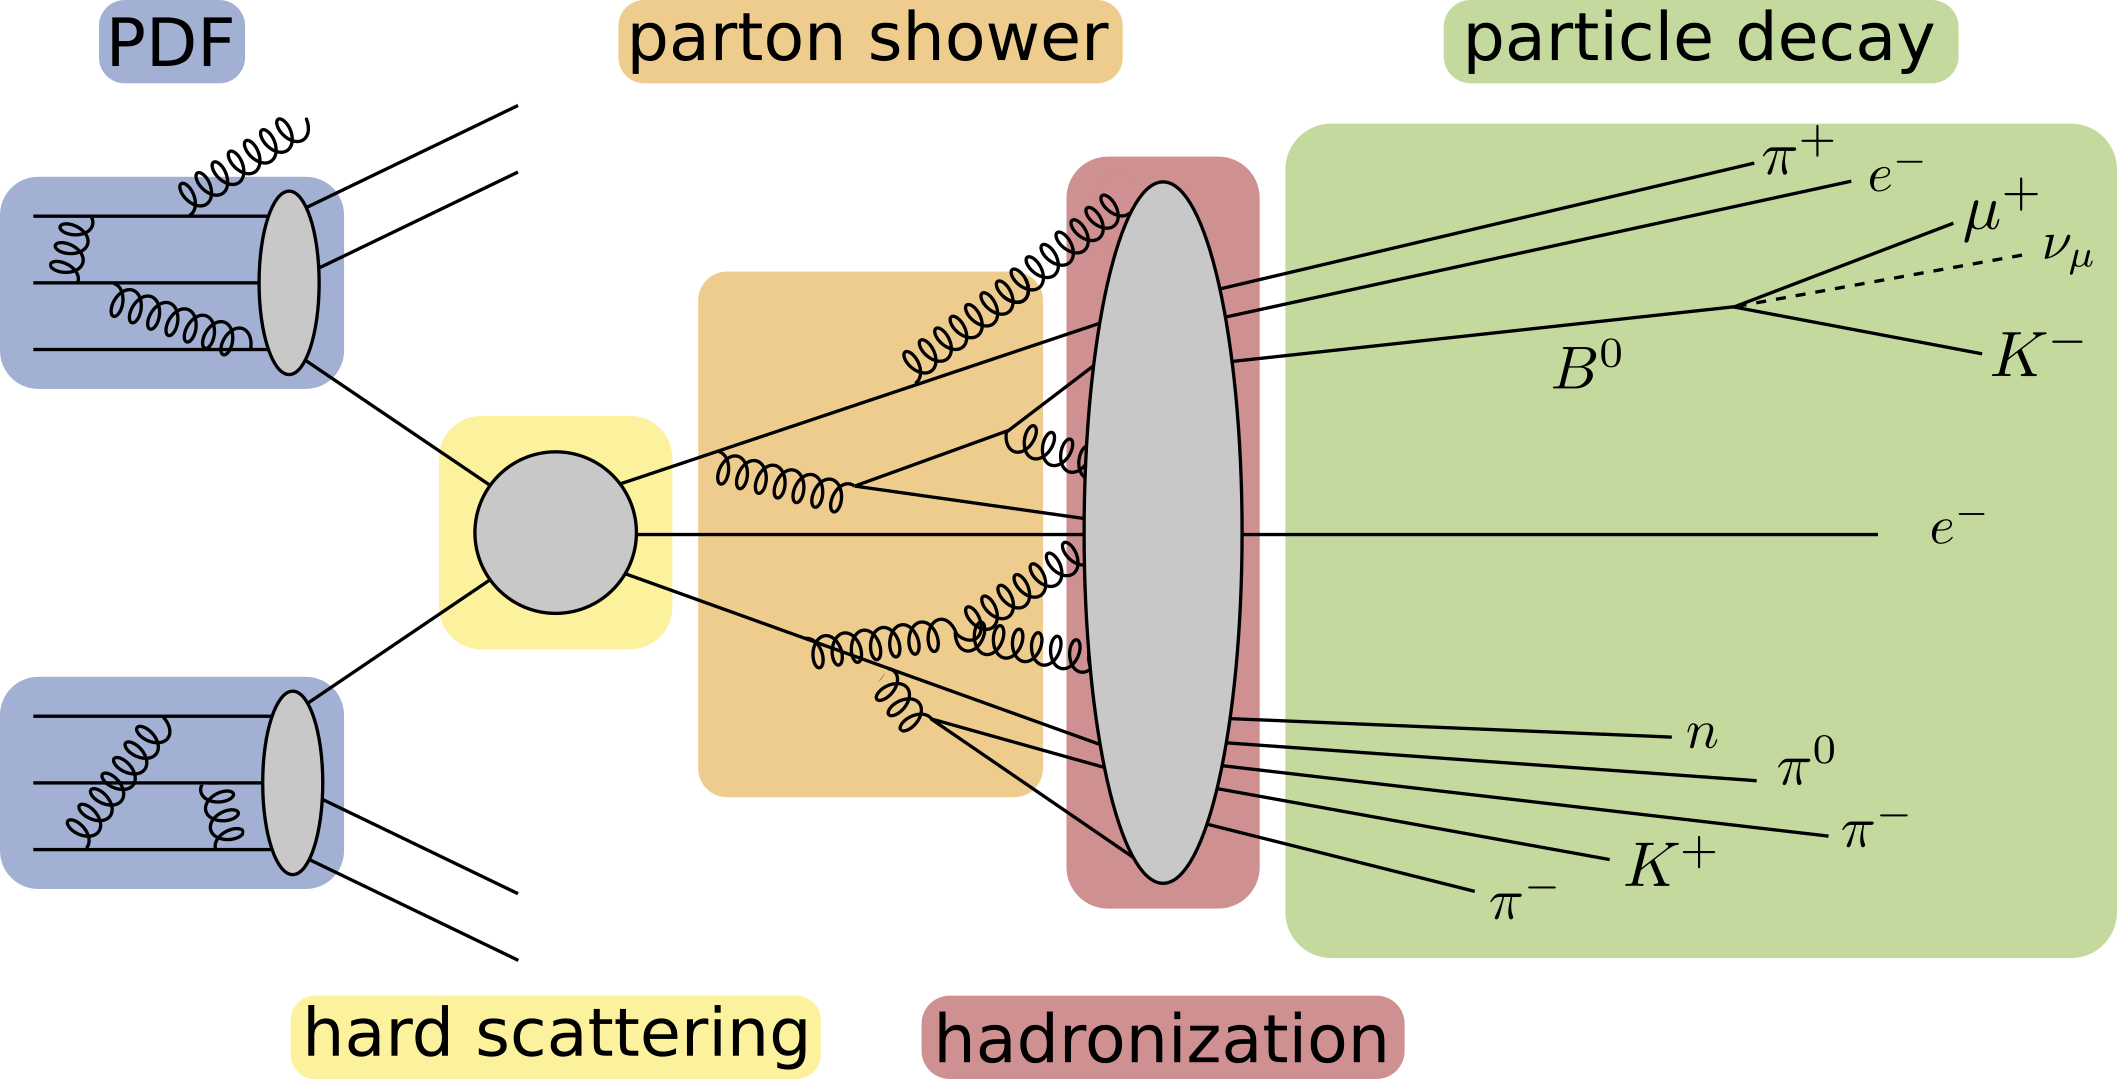
\includegraphics[width=0.8\textwidth]{chapter_3_gen/scattering.png}
\caption[Proton-Proton Scattering Process]{\textbf{Proton-proton scattering process:} The parton distribution functions (PDF) describe how the constituents of the proton are distributed. The deep inelastic scattering process of two elementary particles is calculated in the hard scattering. The subsequent processes are the parton shower, the hadronization and the particle decay.}
\label{fig:ch_3_scattering}
\end{figure}

\subsubsection*{Parton Distribution Functions}
As described in section \ref{sec:ch_1_QCD}, the proton is not an elementary particle but consists of so called partons. The valence quarks (uud) determine the quantum numbers of the proton. Apart from these, also gluons exist inside of protons as they are the exchange particles of the strong interaction. The gluons can split into virtual quark-antiquark-pairs; these quarks are the so called sea quarks. In a deep inelastic proton-proton scattering, two partons from two colliding protons interact with each other. Each parton carries a momentum fraction $x$ of the proton. The probability that a specific parton interacts, depends on $x$ and the absolute transfered momentum $Q$. It is given by a parton distribution function (PDF). As the PDFs cannot be computed by perturbation theory, they are determined by global fits to data from electron-proton scattering, fixed target experiments or hadron colliders. A classic approach is a polynomial ansatz for a specific PDF \cite{pdfOld}. A more modern approach is using a three-layer feed-forward neural network with 37 parameters \cite{nnpdf}. One can define a factorization scale $\mu$ and absorb low energetic gluons into the PDF, thereby infrared divergences are avoided. The use of the Dokshitzer-Gribov-Lipatov-Altarelli-Parisi (DGLAP)-equations \cite{DGLAP1,DGLAP2,DGLAP3} allows the evolution of gluon and quark PDFs to a desired value of $Q$. The PDFs for two different values of $\mu$ are shown in figure \ref{fig:ch_3_pdfs}.

\begin{figure}
%\hfill
%\subfigure{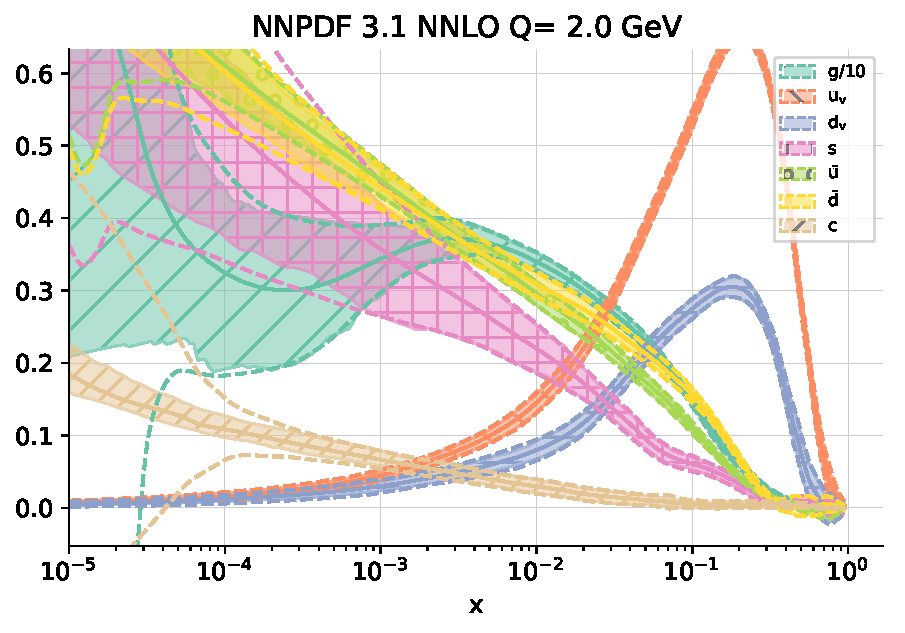
\includegraphics[width=7.25cm]{chapter_3_gen/NNPDF31NNLO_10GeV.pdf}}
%\hfill
%\subfigure{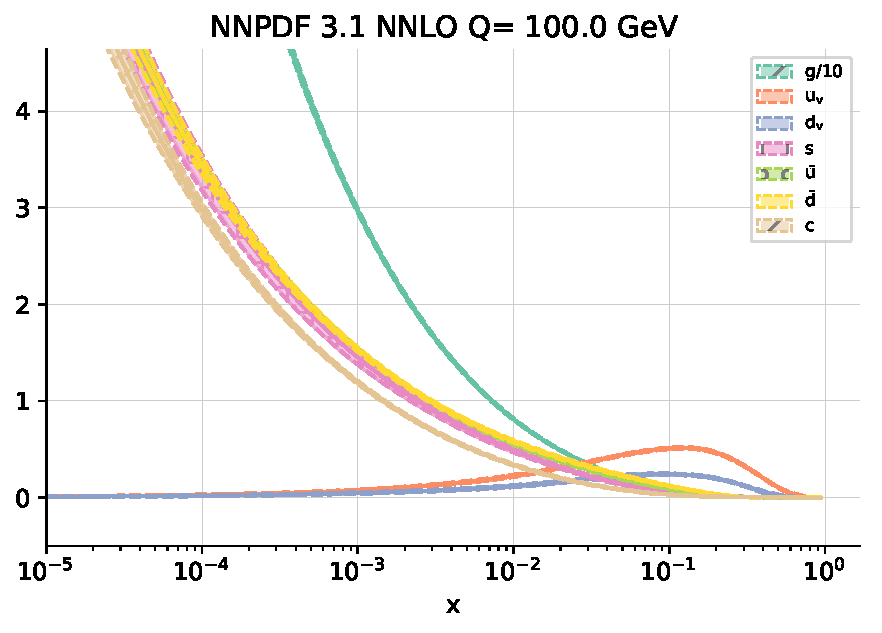
\includegraphics[width=7.25cm]{chapter_3_gen/NNPDF31NNLO_100GeV.pdf}}
%\hfill
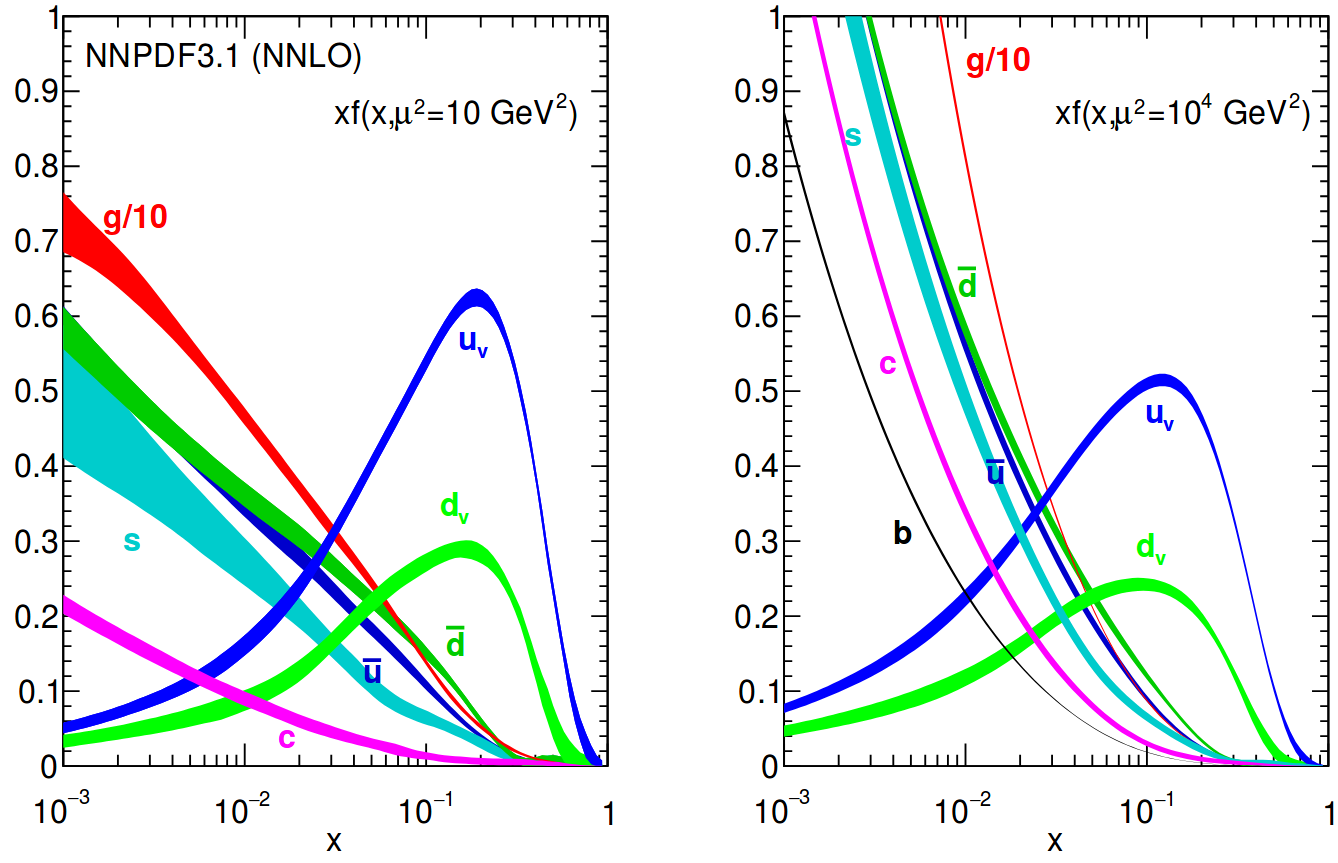
\includegraphics[width=0.75\textwidth]{chapter_3_gen/nnpdfs.png}
\caption[Parton Distribution Functions]{\textbf{Neural Network Parton Distribution Functions (NNPDFs).} Shown are the PDFs of gluons, valence quarks and sea quarks for different momentum fractions $x$ of the proton momentum. At lower values of the factorization scale (left) the valence quarks carry the majority of the proton momentum. At higher values of factorization scale (right) gluons carry the dominant part. The PDFs are computed using the DGLAP-equations in next-to-next-to-leading-order (NNLO). Source: \cite{nnpdf}}
   \label{fig:ch_3_pdfs}
\end{figure}

\subsubsection*{Hard Scattering Process}
The differential cross section $\textrm{d}\sigma$ for the hard scattering process is weighted with the PDFs $f_{i,j}$, which give the probabilities to find certain partons with certain momentum fractions $x$ and $y$ of the colliding protons. It is given by
\begin{equation} \label{eq:ch_3_sigma}
\textrm{d}\sigma = \frac{1}{3}\ \sum_{i,j}\ f_i(x,\mu^2)\ f_j(y,\mu^2)\ \frac{1}{2(xys)^2}\ |\mathcal{M}_{i,j \rightarrow \textrm{final}}|\ \frac{\textrm{d} \cos \theta\ \textrm{d}\phi\ \textrm{d}x\ \textrm{d}y}{8(2\uppi)^2} \quad ,
\end{equation}
with the square of the center-of-mass energy $s$ and the transition amplitude $\mathcal{M}_{i,j \rightarrow \textrm{final}}$ for an initial state to a final state, the so called matrix element. $\mathcal{M}_{i,j \rightarrow \textrm{final}}$ is obtained by summing up all Feynman diagrams for a specific process in a perturbation series. This is possible because the momentum of the partons is in a regime where $\alpha_s \ll 1$ and convergence of the series is given. Often it is sufficient to take the leading order (LO) Feynman diagrams, which are the ones with the minimal amount of vertices that are needed for a specific process. Including next-to-leading order (NLO) Feynman diagrams improves the accuracy of the simulation but is more complex and computationally intensive in generation.\\

The simulation is done with the help of Monte Carlo (MC) methods \cite{MCmethod}. MC methods can be used for numerical integration of higher dimensional phase spaces. In principle, to obtain one simulated event that obeys equation \ref{eq:ch_3_sigma}, the following can be done \cite[p. 48]{PPscattering}. Uniform distributed random numbers ($\theta,\ \phi,\ x,\ y,\ i,\ j$) are taken in the corresponding value ranges and $\left<\mathrm{d}\sigma\right>$ is calculated at one specific phase space point. The event is further processed if another uniform distributed random number $g$ in the range 0 < $g$ < $\mathrm{d}\sigma_\textrm{max}$ is lower than $\left<\mathrm{d}\sigma\right>$, where $\mathrm{d}\sigma_\textrm{max}$ is the supremum of $\mathrm{d}\sigma$. Otherwise it is discarded. Repeating this procedure equals an integration of the total phase space of equation \ref{eq:ch_3_sigma}.\\


\subsubsection*{Parton Shower, Hadronization and Particle Decay}
In addition to the final state particles of the hard scattering process, gluons and photons can be produced in initial or final state radiation. Gluons can radiate off another gluon or split into quark-antiquark pairs; photons can split into fermion pairs. These processes can recur and are described by the DGLAP-equations. A so called parton shower emerges. Because of the confinement (section \ref{sec:ch_1_QCD}), the partons form hadrons. This process cannot be described in a perturbation series as the assumption of $\alpha_s \ll 1$ does not hold for lower energies of the partons. The effect is described by phenomenological models like the Lund string model \cite{LundString}. The hadrons can further decay, as most of them are unstable. 

\subsubsection*{Underlying Event and Pileup}
Besides the hard scattering process of two partons, the remaining partons can interact themselves, producing additional signals in the detector at the same time. This effect is called underlying event. In the same bunch crossing, several other proton pairs are interacting with each other, this is called in-time pileup. Out-of-time pileup considers previous bunch crossings. The pileup distribution depends on the collider's properties. The more protons are in one bunch and the more focused the beams are, the more pileup events happen. In the data recorded in 2016, there were in average about 27 pileup events per bunch crossing in the CMS detector \cite{lhclumi2016}. The pileup events can be simulated as additional random scatterings and merged with the main event. 

\subsection{Simulation Tools} \label{sec:ch_3_simtools}
In the event simulation, several tools are used for the different steps. For the matrix element, one common generator is \textsc{MadGraph5} \cite{MadGraph5}. It sums up all Feynman diagrams in LO for given initial and final state particles. The matrix element is generated but not evaluated yet. The evaluation is done with the \textsc{MadEvent} package \cite{MadEvent} at given phase space points with the MC method and the cross section is calculated. For this reason a simulated event is often called MC event. \\

\textsc{MadGraph5}\textunderscore \textsc{aMC@NLO} \cite{MadGraph5_NLO}  is a further developement of \textsc{MadGraph5}, combining the features of MadGraph5 with the ones of \textsc{aMC@NLO}, where \textsc{aMC@NLO} can generate matrix elements at NLO in QCD. These tools also provide different parton-shower matching schemes to combine the final state particles with the parton shower. The parton shower itself has to be added with a parton shower simulation tool. As explained earlier, the parton shower can cause additional gluons in the final state, but such gluons can also be produced in NLO matrix element generators. To avoid double counting, the parts of the parton shower that match the NLO Feynman diagrams are subtracted. This is implemented by using negative event weights.\\

Another matrix element generator that includes Feynman diagrams up to NLO in QCD is \textsc{Powheg} \cite{Powheg1, Powheg2, Powheg3}. \textsc{Powheg} uses a different method than \textsc{aMC@NLO} to avoid double counting and negative event weights. It demands a parton shower simulation that generates the emission with the highest \pt first and then corrects the NLO emission. \\

\textsc{Pythia} \cite{Pythia82} is a general purpose tool for the simulation of the hard process as well as the parton shower, the hadronization, the particle decay and the underlying event. The hard process is only calculated in LO, but \textsc{Pythia} provides several interfaces to external programs. Therefore, the matrix element generators explained above can be used in combination with \textsc{Pythia}. \\

To be able to compare simulation with data, the detector response has to be simulated as well. This is done with the \textsc{GEANT4}\cite{Geant4} toolkit. In \textsc{GEANT4}, the different materials of the detector system, including dead materials, are modeled. The particles are propagated through these materials while taking into account the effect of the magnetic field on charged particles. Interactions like bremsstrahlung, multiple scattering and photon pair-production are simulated. The generated signals in the active detector materials are taken as input for emulators of readout electronics and trigger systems. After this step, the detector information of a simulated event is in the same manner as for data. To get the best comparison between data and simulation, the event reconstruction of the detector signals is done in the same way as for data. This will be subject of the next section.


\section{Event Reconstruction}
In this chapter, the aim to reconstruct physics objects out of the measured or simulated detector information is described. In a first step of the event reconstruction, particle tracks and the corresponding interaction points, called vertices, are reconstructed. In several subsequent steps, the identification and reconstruction of particles that penetrate the detector is done. These are electrons, muons, photons, charged hadrons, neutral hadrons and neutrinos. Afterwards, adjacent particles are bundled to so called jets. 

\subsection{Tracks and Vertices}
Tracks of charged particles are reconstructed from the tracker information. Therefore, tracker hits are created from clustering signals of the silicon pixel and strip detectors. The tracks are produced using an iterative track finding algorithm. From tracker hits in the inside of the detector, where the occupancy of each detector element is low, tracker seeds are created. The track finding is performed with the Kalman filter approach \cite{KalmanFilter}. In the first iteration step, the seeds have tight constrains. This gives only a moderate efficiency, but also a minimal fake rate. The energy deposits of the corresponding hits are then removed, which simplifies the track finding problem. At the next iteration step with looser seeding criteria, a higher efficiency is achieved. Repeating this, one gets an efficiency to find isolated muons of 99.5\% and more than 90\% to find charged hadrons while the fake rate is of about 1\% \cite{ParticleFlow2}. Each track has several quality criteria like the number of hits, a normalized $\upchi^2$ value and the compatibility to a certain vertex.\\

Because of pileup, there exists more than one vertex for each event. The vertex from where the hard scattering originates is the primary vertex (PI), it has to be identified in order to remove the tracks originating from pileup. The vertex reconstruction starts with a set of possible vertices and each track is extrapolated to a point $z_i$ on the beam line. For each track and vertex pair a probability $c_{ik}$ is estimated that the track is originating from the regarded vertex. A $\upchi^2$ function, weighted with these probabilities
\begin{equation}
\chi^2 = \sum_{i,k} c_{ik} \frac{(z_i-z_k)^2}{\sigma_i^2}	\quad ,	
\end{equation}
is minimized to determine the exact position of the vertices $z_k$. As the probability depends on the vertex position, an iterative procedure is used. After a final selection, a set of vertices is obtained. The primary vertex is selected as the one with the highest sum of $p_\textrm{T}^2$ of its tracks. 

\subsection{Particle Reconstruction}
For reconstructing particles as precise as possible, the combination of all subdetectors is used within the particle flow (PF) algorithm \cite{ParticleFlow, ParticleFlow2}. The identification of PF candidates, namely electrons, muons, photons, charged hadrons and neutral hadrons is explained in the following. 

\subsubsection*{Calorimeter Clustering}
The tracker system gives the most precise information about the position and through the curvature of the track, it gives also the best determination of the momentum of charged particles. The calorimeters support the determination of the energy and direction of charged particles in cases of high \pt or low quality tracks. Moreover the energy and direction of photons and neutral hadrons is measured while the contributions of charged particles are separated. This is done in the calorimeter clustering process, where each calorimeter element, the ECAL barrel, the ECAL endcap and the several HCAL elements, are handled separately. The process starts on calorimeter cells with a local maximum of deposited energy. Then, adjacent cells are combined, if their deposited energy exceeds a certain threshold. For each calorimeter element, one can have several calorimeter clusters. Together with the charged-particle tracks and the muon tracks, PF elements can be constructed.

\subsubsection*{Electrons}
An electron is identified if a charged-particle track matches an ECAL cluster with a typical electron shower profile. A fit starting with a track seed is combining both signals and the momentum is determined. A complimentary algorithm for electrons with high \pt starts with taking a seed from the ECAL. In this algorithm, several ECAL clusters are combined to so called ECAL superclusters which have a characteristic form for electrons \ref{ERec}. The quality of an electron fit is described by several quantities like the matching of the track to the cluster or the distance of the track to the primary vertex. A tight requirement on these quantities can lower the fake rate.

\subsubsection*{Muons}
For the muon reconstruction, tracks in the muon chamber are computed in a similar way as in the tracker. These muon tracks are propagated towards the beam line and combined if possible with the most suitable track of the inner tracker. A refit using the information of both sub detectors gives an improved muon track. A reconstruction process for low \pt muons that do not create a muon track, starts with propagating an inner tracker track and tries to find a minimal muon information in the muon tracker. Again one can choose looser or tighter demands on muon tracks afterwards to further reduce the fake rate.

\subsubsection*{Hadrons and Photons}
For the reconstruction of charged hadrons, the energy depositions of clusters in ECAL and HCAL are compared to the momentum of the charged particle tracks. In case of an agreement with one or more tracks, a combined fit is performed. In case of disagreement, several scenarios including additional neutral hadrons or photons are considered. After all charged-particle tracks are matched to PF elements, their energy deposits are removed and neutral particles are identified. Neutral particles do not produce any hits in the tracker, therefore they have only bad direction information and an assignment to a vertex is not possible. Because of this, also neutral particles coming from pileup are included.

\subsection{Jet Reconstruction}
A jet is a particle shower of hadrons, leptons and photons that originates in the most cases from a single particle. There are different ways to reconstruct a jet, the default method used in the CMS experiment collects several nearby PF elements in a cone up to a given size in a sequential recombination process. This is done with the anti-$k_\textrm{t}$ jet clustering algorithm \cite{antikt}. \\

\begin{figure}
\centering
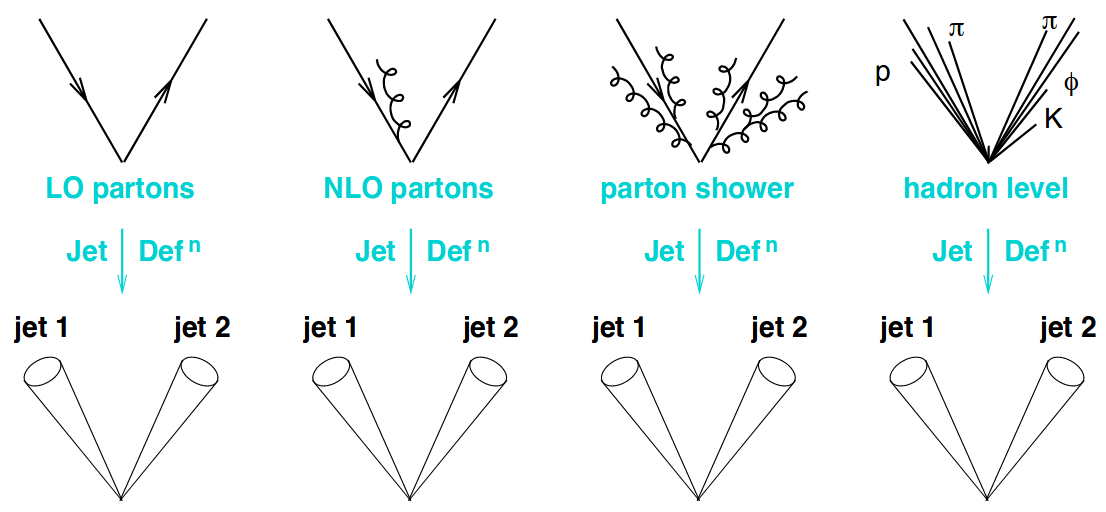
\includegraphics[width=0.75\textwidth]{chapter_3_gen/IRCsafety.png}
\caption[Infrared and Collinear Safety of Jets]{\textbf{Infrared and collinear safety.} A jet can be defined on different levels. In a theoretical description, it originates from one single particle and can therefore defined as this particle. In perturbation theory, several vector bosons can be radiated in addition. On the detector level, the jet is defined by color neutral objects. With an infrared and collinear safe jet clustering algorithm, the resulting jets are independent of the level of definition. Source: \cite{ICLsafe}}
\label{fig:ch_3_IRCsafety}
\end{figure}

An advantage of this algorithm is its infrared and collinear safety. This means, that the same jet is found with and without a soft or collinear radiation, for example a gluon radiation or a gluon splitting. Therefore, this algorithm is independent of the technical level of the jet definition as shown in figure \ref{fig:ch_3_IRCsafety}. For the clustering process, a distance measure $d_{ij}$ between two particles $i$ and $j$ is defined as
\begin{equation}
d_{ij} = \textrm{min}(k_{\textrm{t},i}^{-2},k_{\textrm{t},j}^{-2})\frac{\Delta R^2_{ij}}{R^2} \quad ,
\end{equation}
where $k_{\textrm{t},i}$ is the momentum of a particle, $R^2 = (y^2 + \phi^2)$ is the radius in the $y$-$\phi$ plane with the rapidity $y$ and $\Delta R^2_{ij} = (y_i - y_j)^2 + (\phi_i - \phi_j)^2$ is a radial distance of two particles. A distance measure $ d_{i\textrm{B}}$ between a particle $i$ and the beam axis is defined as
\begin{equation}
d_{i\textrm{B}} = k^{-2}_{\textrm{t},i} \quad .
\end{equation}
For the general jet reconstruction of data taken from run 2 of the CMS experiment, a radius of $R=0.4$ was chosen. In the sequential recombination algorithm, all possible $d_{ij}$ are computed and two particles with the smallest $d_{ij}$ are combined to new pseudo-particles. This is repeated until $d_{i\textrm{B}}$ is the smallest distance. The remaining pseudo-particles become then the jets. In this way, the hardest particles (the ones with the highest \pt) are combined with nearby soft particles (the ones with low \pt). If the cones of two hard particles overlap, they share the softest particles and create two separate jets with partial cones. 

\subsection{Lepton Isolation}\label{sec:ch_3:Isolation}
Muons and electrons often appear inside of QCD jets originating from b, c or s quark decays. Isolated leptons on the other hand appear often in rare processes, they are good indicators for leptonic top quark decays ($ \textrm{t} \rightarrow \textrm{b} + \upnu_l + l^+$). Therefore an isolation criteria is useful to find events with bottom quarks without directly looking at them. An isolation can be described using the momenta and energies $p_\textrm{T}^\textrm{charged}$, $E_\textrm{T}^\textrm{neutral}$ and $E_\textrm{T}^\upgamma$ of the PF elements for the charged particles, the neutral particles and the photons respectively inside a cone of 
\begin{equation}
\Delta R = \sqrt{\Delta\eta^2 + \Delta\phi^2} = 0.4 \quad .
\end{equation}
Since the tauon decays in the beam line, only for an electron or a muon with its momentum $p_\textrm{T}^l$ an isolation can be defined as
\begin{equation}
I_l^{\textrm{PF}/\Delta \upbeta} = \frac{\sum p_\textrm{T}^\textrm{charged} + \textrm{max} \left(0.0, E_\textrm{T}^\textrm{neutral} + \sum E_\textrm{T}^\upgamma - 0.5 \sum E_\textrm{T}^\textrm{charged}(\textrm{PU})\right) }{p_\textrm{T}^l} \quad .
\end{equation}
The so called $\Delta \upbeta$ correction is included where contributions of the neutral particles from pileup interactions are subtracted. They are estimated as half of the energy coming from charged particles in pileup $\sum E_\textrm{T}^\textrm{charged}(\textrm{PU})$. A lower value of $I_l^{\textrm{PF}/\Delta \upbeta}$ corresponds to a more isolated electron or muon.  


\subsection{Reconstruction of Neutrinos and Leptonically Decaying W Bosons}
At the LHC, the transverse momentum $\vec{p}_\textrm{T} = (p_x, p_y)^\textrm{T}$ of the colliding particles is zero, therefore the sum of the $\vec{p}_\textrm{T}$ of all generated particles after the collision has to be zero as well. As neutrinos cannot be measured within the CMS detector the missing part of the transverse momentum can be attributed to neutrinos. For historical reasons and as the momentum is equal to the energy in the relativistic regime using natural units, the missing part is denoted as the missing transverse energy 
\begin{equation}
\vec{\slashed{E}}_T = - \sum_i \vec{p}_{\textrm{T},i} \quad .
\end{equation}
Decays of the W boson into a charged lepton and a neutrino are called leptonic W boson decays. With the measured $\vec{\slashed{E}}_T$ and the momentum of the lepton, the transverse mass of the W boson $m_{\textrm{T,W}}$ can be reconstructed 
\begin{equation}
m_{\textrm{T,W}} = \sqrt{(\vec{p}_{\textrm{T},l} + \vec{p}_{\textrm{T},\nu})^2 - (p_{x,l} + p_{x,\nu})^2 - (p_{y,l} + p_{y,\nu})^2} \quad ,
\end{equation}
with $\vec{p}_{\textrm{T},\nu}$ the neutrino momentum set to $\vec{\slashed{E}}_T $. This method allows to reconstruct the W boson if there are no additional W bosons or leptons in the event.

\section{Differences between Data and Simulation} \label{sec:ch_3_Reweighting}
As mentioned before, the simulation is not exact since in each step smaller or larger inaccuracies are made. These differences lead to discrepancies between data and simulation after the reconstruction. Several steps can be done to improve the agreement afterwards, these are explained in the following.

\subsection{Jet Energy Corrections}
In general, the measured jet energy does not match the true parton energy, where the jet originated from. One reason is pileup and underlying events. Due to the tracks, the charged particles from pileup can be removed reasonably well but the neutral particles not. Also neutrinos are not measured and they appear also in jets, therefore, their energy is missing. Moreover, there is a disagreement in data compared to simulation due to inaccuracies in the simulation. With jet energy corrections (JEC) \cite{JEC}, these differences are mitigated in several steps with some variation for data and simulation. These steps are outlined in figure \ref{fig:ch_3_JEC}.

\begin{figure}
\centering
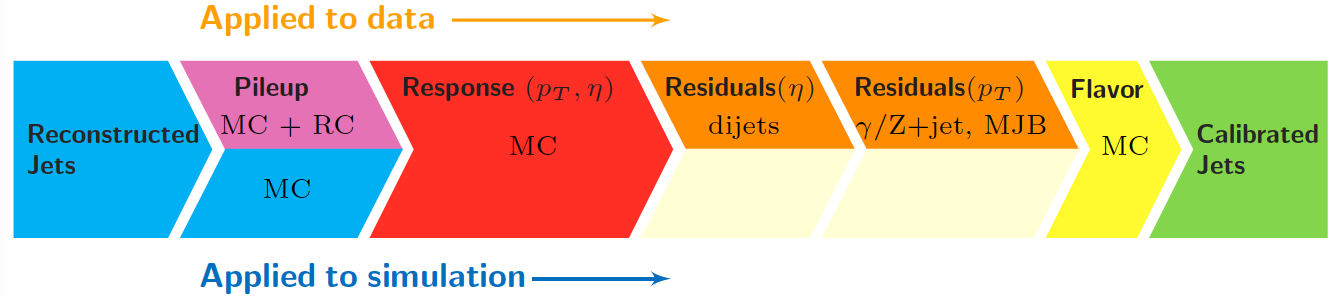
\includegraphics[width=0.95\textwidth]{chapter_3_gen/JEC_levels.png}
\caption[Jet Energy Corrections]{\textbf{Jet Energy Corrections.} In the first step, based on information from simulation, energy contributions from pileup and electronics noise are removed. In data, the residual differences between data and simulation as a function of $\eta$ is flattened as well. Next, the response of the detector is corrected. Therefore, the residual differences in simulation between the reconstructed \pt and $\eta$ and the corresponding true values are flattened out. The resulting correction is performed in data and simulation. A further step is done only on data, here small residual differences between data and simulation in \pt and $\eta$ are corrected. An optional last step is the correction in dependence of the flavor of the jet using the truth information from the simulation. Source: \cite{JEC_levels}}
\label{fig:ch_3_JEC}
\end{figure}

\subsection{Pileup Reweighting}
The simulation is done before or during the actual data taking period, therefore a pileup distribution has to be assumed in the simulation. To correct most of the disagreements caused by the different pileup interactions, the simulated events can be assigned with a weight in a way that the pileup distributions in data and simulation are equal. The pileup weights are given by 
\begin{equation}
w_{\textrm{PU},i} = \frac{n_{\textrm{data},i}}{n_{\textrm{MC},i}} \quad ,
\end{equation}
with the number of data events $n_{\textrm{data},i}$ and the number of simulated events $n_{\textrm{MC},i}$ in dependency of the number of primary vertices $i$. The pileup distributions for the 2016 data and simulation are shown in figure \ref{fig:ch_3_pup}. 

\begin{figure}
\centering
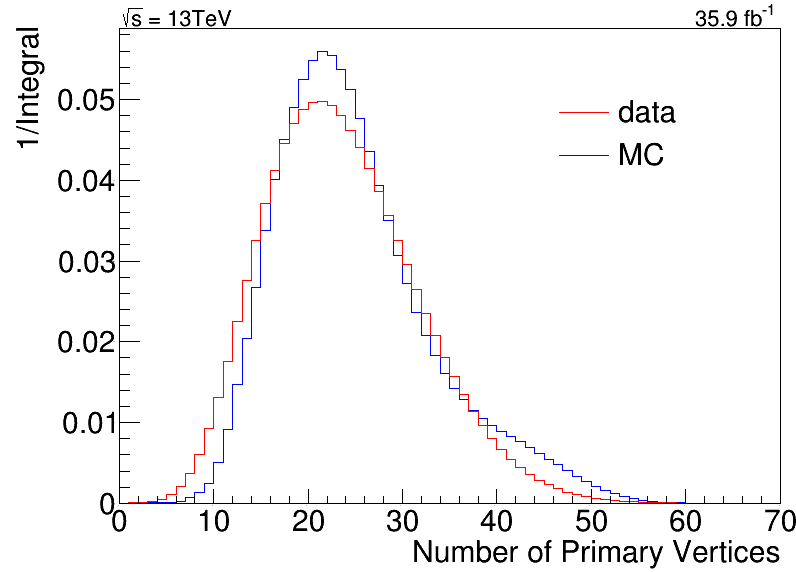
\includegraphics[width=0.5\textwidth]{chapter_3_gen/pup.png}
\caption[Pileup Distributions for Data and Simulation]{\textbf{Pileup distribution for data and simulation.} Shown is a normalized histogram of the events as a function of the number of primary vertices. In each bin where the data is above the simulation, the simulation gets up-weighted; when the data is lower than the simulation, the simulation gets down-weighted.}
\label{fig:ch_3_pup}
\end{figure}

\subsection{Trigger and Lepton Efficiencies}
The efficiency of the triggers is also different in data and simulation. In order to mitigate this discrepancy, scalefactors are used to correct the simulation
\begin{equation}
sf_\textrm{trigger} = \frac{\epsilon_\textrm{data}(\pt,\eta,\dots)}{\epsilon_\textrm{MC}(\pt,\eta,\dots)} \quad ,
\end{equation}
where the efficiencies $\epsilon_\textrm{data,MC}$ are functions of different quantities. For example a muon trigger has a strong dependency on the \pt of the corresponding muon. \\

Lepton scalefactors are needed whenever a selection of leptons is performed as the efficiencies of the identification of a lepton are different in data and simulation. The efficiencies are moreover dependent of the selection of the lepton, they are often separated for different parts of the selection (for example for the tracker selection and the isolation criteria) and can be combined. For some selection criteria, scalefactors are already measured.




